\documentclass{article}
\usepackage[utf8]{inputenc}
\usepackage[french]{babel}
\usepackage[T1]{fontenc}
\usepackage{tcolorbox}
\usepackage[margin=2cm]{geometry}
\usepackage{array}
\usepackage{hyperref}
\usepackage{tikz}
\usepackage{listings}
\usepackage{eurosym}
\usepackage{amsfonts}
\usepackage{amsmath}
\usepackage{cancel}
\usepackage{pdfpages}

\title{IFT2015 automne 2016 - Devoir1} %trouver long trait d'union
\author{Philippe Caron}
\date{\today}

\renewcommand{\thesubsubsection}{\alph{subsubsection}.}
\renewcommand{\thefootnote}{\fnsymbol{footnote}}
\newenvironment{pseudo}{\begin{tcolorbox}[left skip = 1cm, right skip = 1cm]}{\end{tcolorbox}}
\newcommand{\key}[1]{{\bf #1}}
\newcommand{\name}[1]{{\scshape #1}}
\newcommand\tab[1][0.5cm]{\hspace*{#1}}

\lstset{frame=tb,
  language=Python,
  aboveskip=3mm,
  belowskip=3mm,
  showstringspaces=false,
  columns=flexible,
  basicstyle={\small\ttfamily},
  numbers=none,
  numberstyle=\tiny\color{pink},
  keywordstyle=\color{purple},
  commentstyle=\color{dkgreen},
  stringstyle=\color{brown},
  breaklines=true,
  breakatwhitespace=true,
  tabsize=3
}

\begin{document}
\maketitle
\section{Tableaux de hachage}
En premier lieu, il fallait s'assurer de pouvoir supporter \texttt{null}, pour ce faire il a suffit d'étendre la classe \texttt{LinearProbing} et de remplacer l'élément nul par un nouvel objet, nommé \texttt{VOID}. Puis il suffit de modifier les fonctions qui utilisaient \texttt{null} pour supporter le nouvel élément nul, ce qui a donner la classe \texttt{NLinearProbing} de laquelle découlent les deux prochaines classes.
\subsection{Suppression paresseuse}
Nommée \texttt{LazySet}, la classe qui permet la suppression paresseuse hérite de \texttt{NLinearProbing}. La différence principale est l'utilisation de la «pierre tombale» \texttt{DELETED} pour la suppression. Ceci permet d'implémenter \texttt{remove}, qui permet de retirer un élément du tableau et de réduire sa taille lorsqu'il descend sous un certain facteur. Il a également fallu modifier \texttt{add} pour accomoder le nouvel object \texttt{DELETED}. Pour se faire la nouvelle fonction \texttt{searchDel} a été créée. Elle est essentiellement identique à \texttt{search} cependant elle cherche aussi les cases supprimées ce qui permet de recycler les cases supprimées.
\subsection{Suppression impatiente}
La classe nommée \texttt{HastySet} implémente un tableau de hachage supportant la suppression impatiente. Tout comme la précédente, elle hérite de \texttt{NLinearProbing} afin de supporter les éléments null. Vu que cette classe déplace les éléments vers l'avant après une suppression, elle ne nécéssite pas que ses méthodes de recherche et d'ajout soient supprimées. La seule méthodes implémentées est donc \texttt{remove}. Elle fonctionne de la même manière que celle de la suppression paresseuse au nouveau du \textit{rehash}, mais au lieu de remplacer l'élément supprimé par un marqueur, elle déplace tous les éléments subséquents vers l'avant.
\section{Résultats}
Le fichier de résultat a été produit à l'aide de la commande suivante:
\begin{pseudo}
  \texttt{\% bash -c 'for t in Hash Lazy Hasty; do for N in 65536 131072 262144 524288 1048576 2097152 4194304; do for rep in 1 2 3 4 5 6 7 8 9 10 11 12; do java -Xmx2G -cp dev4.jar SetTester -type \$\{t\} \$\{N\}; done; done; done' > timings.log}
\end{pseudo}
Pour chaque type, toutes les tailles sont testées, et pour chaque taille le test est effectué 12 fois. Voici les spécifications de la machine de test:
\begin{verbatim}
Machine : Laptop Lenovo IdeaPad
Mémoire : 8GB
Processeur : Intel i7 @ 2.7 GHz (8 Threads / Quad Core)
OS : ARCH Linux 4.7.6-1
Java: OpenJDK 64-Bit Server VM 25.102-b14 (1.8.0_102-b14)
\end{verbatim}
Les graphiques obtenus sont à la page suivante.
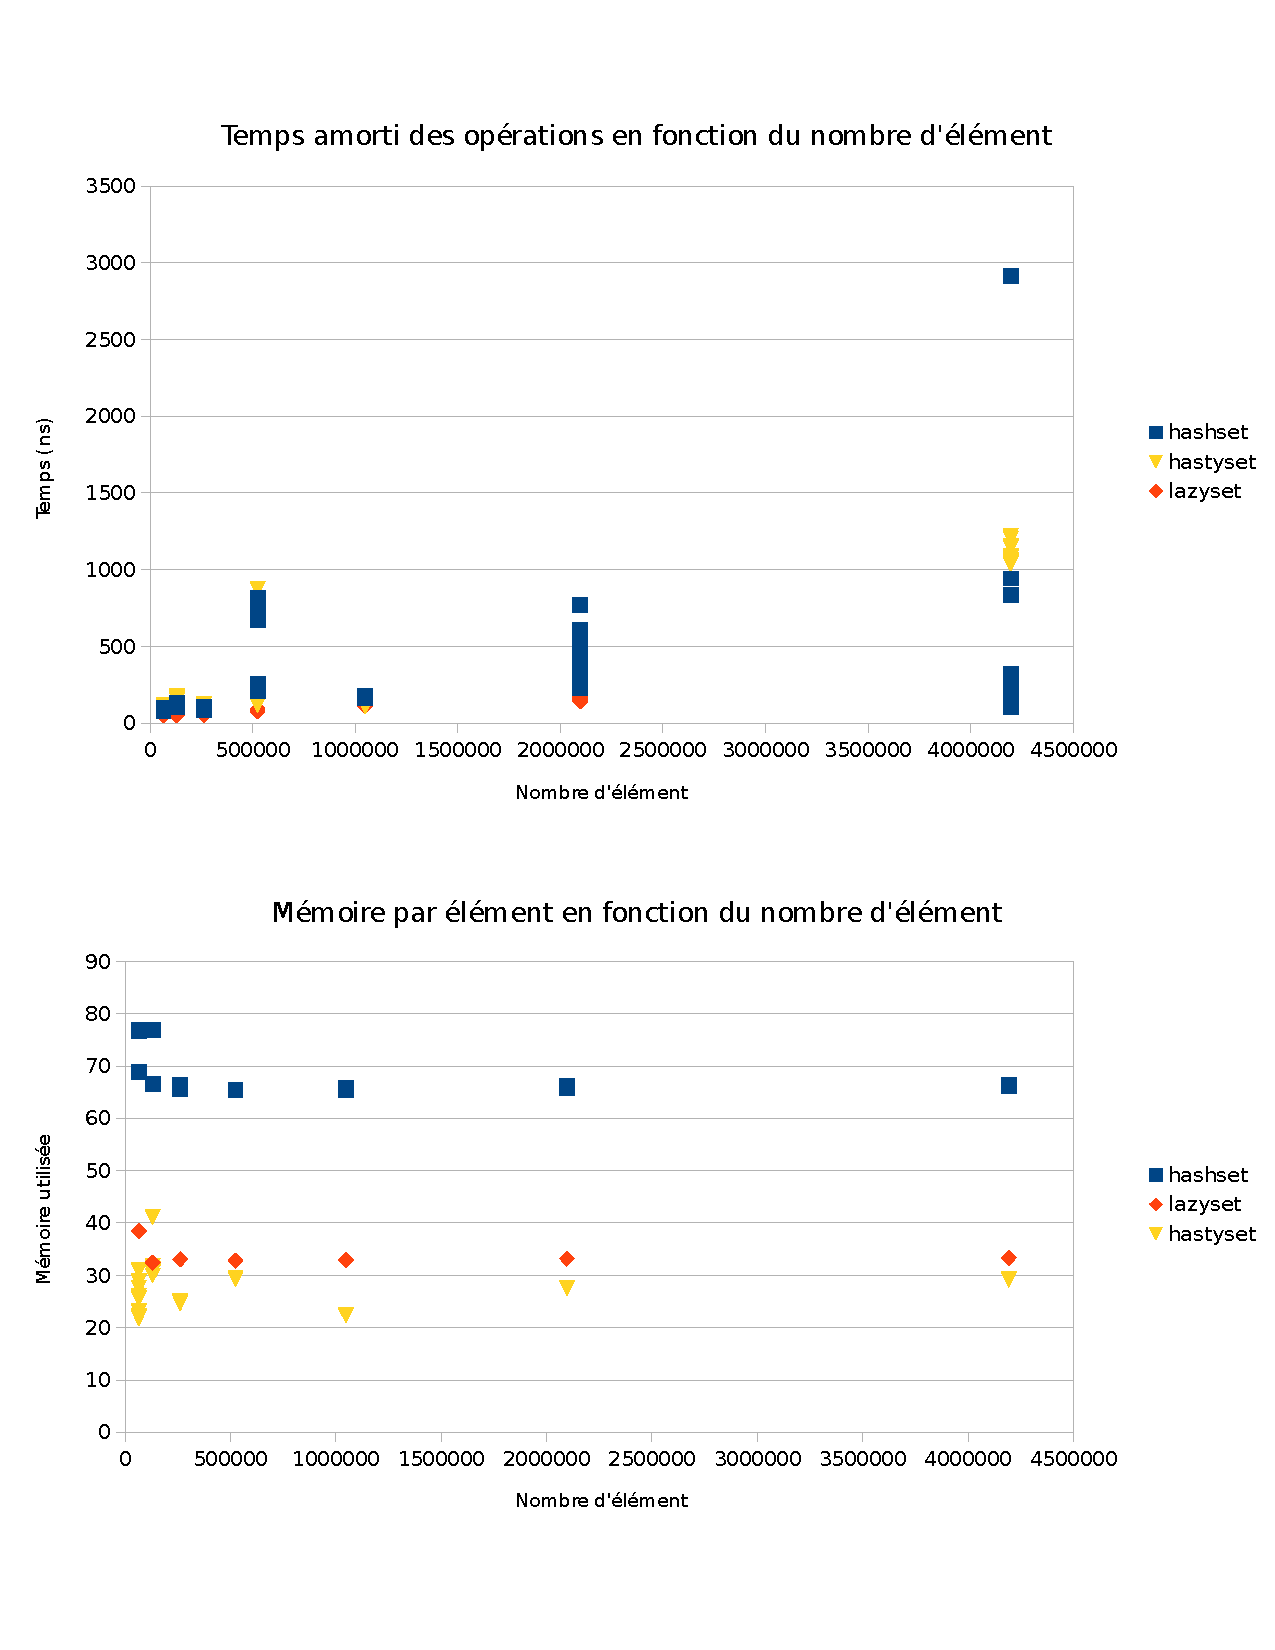
\includepdf[page=-]{stats.pdf}
\subsection{Vitesse}
On peut voir qu'au niveau de la vitesse les trois implémentations sont très similaires, cependant on remarque toutefois que la suppression impatiente tend à prendre plus de temps dans les tableau qui présentent un grand nombre d'élément. La suppression paresseuse quant à elle semble légèrement plus efficace que l'implantation \texttt{HashSet} de java, mais c'est négligeable.
\subsection{Mémoire}
Au niveau de la mémoire, les deux implémentations qui héritent de \texttt{NLinearProbing} sont manifestement plus efficaces. Quoique relativement similaires entre elles, chacune prend significativement moins de mémoire que \texttt{HashSet}.
\end{document}
